\section{Data}
This section describes the data used in the study.

\subsection{Mouse models}
Describe the mouse models used in the study and how they were generated.

\subsection{Samples}
Describe the samples used in the study and how they were collected.
Include the timeline plots from the poster.
Explain the different sequencing steps.

\section{Nextflow and nf-core}
\paragraph{Nextflow} is a workflow management system that enables the
development of reproducible and scalable workflows. It allows the creation of
complex pipelines that can be executed on a variety of platforms, from local
machines to cloud computing environments. Nextflow uses a domain-specific
language (DSL) that simplifies the definition of workflows and enables the reuse
of existing components \supercite{di_tommaso_nextflow_2017}. As a result,
Nextflow has become a popular tool in the bioinformatics community.

\begin{figure}[ht]
    \centering
    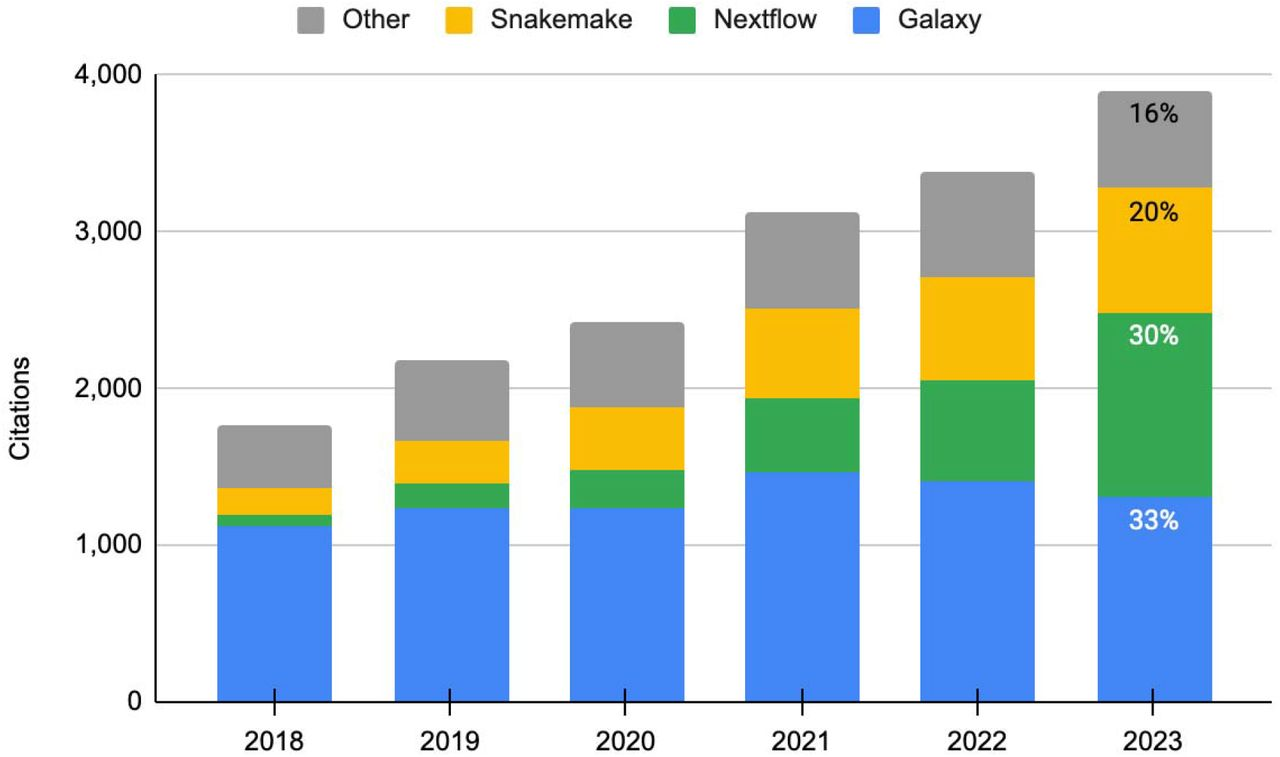
\includegraphics[width=\textwidth]{chapters/materials_and_methods/figures/nextflow_usage.jpg}
    \caption{Workflow management systems} % TODO: Add detailed caption
    \label{fig:nextflow_usage}
\end{figure}

As pointed out by Langer et al. in a recent preprint
\supercite{langer_empowering_2024}, programming-based workflow systems like
Nextflow and Snakemake have gained popularity during the last years, while
GUI-based systems like Galaxy have lost ground. Furthermore, Nextflow has been
the fastest growing workflow system in the last years, with a remarkable 30
percent share of citations in 2023 (\cref{fig:nextflow_usage}). The authors
mostly attribute this to the great quality of the pipelines curated by the
nf-core community \supercite{langer_empowering_2024,grayson_automatic_2023}.

\paragraph{nf-core} is a community-driven project that provides a collection of
high-quality, reproducible, and scalable Nextflow pipelines. These pipelines cover a wide range of
bioinformatics applications, from RNA-seq and ChIP-seq to single-cell RNA-seq
and metagenomics \supercite{ewels_nf-core_2020}.

\section{nf-core/circrna}
High-level overview

\subsection{circRNA detection}
What is the main task here?

\subsubsection{CIRIquant}
Describe CIRIquant

\subsubsection{CIRCexplorer2}
Describe CIRCexplorer2

\subsubsection{circRNA finder}
Describe circRNA finder

\subsubsection{DCC}
Describe DCC

\subsubsection{find circ}
Describe find circ

\subsubsection{MapSplice}
Describe MapSplice

\subsubsection{Segemehl}
Describe Segemehl

\subsection{circRNA annotation}
What is the main task here?

\subsubsection{GTF based annotation}
Describe GTF based annotation

\subsubsection{Database based annotation}
Describe database based annotation

\subsection{circRNA quantification}

Why is this important?

\subsubsection{psirc-quant}
Describe psirc-quant

\subsection{miRNA interaction analysis}
What can we learn from here?

\subsubsection{miRanda}
Describe miRanda

\subsubsection{TargetScan}
Describe TargetScan

\subsection{Downstream analyses}
\subsubsection{R-shiny}
\subsubsection{Dimensionality reduction}
\subsubsection{Pathway analysis}
\subsubsection{Differential expression analysis}
\subsubsection{Genome browser}
